\documentclass[a4paper, 11pt]{article}

\usepackage[margin=3cm]{geometry}
\usepackage[]{fontenc}
\usepackage[utf8]{inputenc}
\usepackage[italian]{babel}
\usepackage{geometry}
\geometry{a4paper, top=2cm, bottom=3cm, left=1.5cm, right=1.5cm, heightrounded, bindingoffset=5mm}
\usepackage{amsmath}
\usepackage{amssymb}
\usepackage{textcomp, gensymb}
\usepackage{graphicx}
\usepackage{psfrag,amsmath,amsfonts,verbatim}
\usepackage{xcolor}
\usepackage{color,soul}
\usepackage{fancyhdr}
\usepackage{indentfirst}
\usepackage{graphicx}
\usepackage{newlfont}
\usepackage{amssymb}
\usepackage{amsmath}
\usepackage{latexsym}
\usepackage{amsthm}
%\usepackage{subfigure}
\usepackage{subcaption}
\usepackage{psfrag}
\usepackage{footnote}
\usepackage{graphics}
\usepackage{color}
\usepackage{hyperref}
\usepackage{tikz}
\usepackage{caption}

\captionsetup[figure]{justification=centering}

\setlength{\parindent}{0pt}

\usetikzlibrary{snakes}
\usetikzlibrary{positioning}
\usetikzlibrary{shapes,arrows}

	
	\tikzstyle{block} = [draw, fill=white, rectangle, 
	minimum height=3em, minimum width=6em]
	\tikzstyle{sum} = [draw, fill=white, circle, node distance=1cm]
	\tikzstyle{input} = [coordinate]
	\tikzstyle{output} = [coordinate]
	\tikzstyle{pinstyle} = [pin edge={to-,thin,black}]

\newcommand{\courseacronym}{CAT}
\newcommand{\coursename}{Controlli Automatici - T}
\newcommand{\tipology}{b }
\newcommand{\trace}{1}
\newcommand{\projectname}{Controllo di meccanismo non-lineare attuato}
\newcommand{\group}{K}

%opening
\title{ \vspace{-1in}
		\huge \strut \coursename \strut 
		\\
		\Large  \strut Progetto Tipologia \tipology - Traccia \trace 
		\\
		\Large  \strut \projectname\strut
		\\
		\Large  \strut Gruppo \group\strut
		\vspace{-0.4cm}
}
\author{Lorenzo Venturoli, Leonardo Benini, Gianluca Sabatini}
\date{}

\begin{document}

\maketitle
\vspace{-0.5cm}

Il progetto riguarda il controllo di un sistema a meccanismo motorizzato di Figura \ref{fig:system_image}, la cui dinamica viene descritta dalle seguenti equazioni differenziali  
%
\begin{subequations}\label{eq:system}
	\begin{align}
		J(\theta)\dot{\omega} = C_m - \beta\omega - k\theta 
	\end{align}
	\begin{align}
		J(\theta) = J_0 + \sum_{n = 0}^{4}J_i\cos (i\theta +\psi_i)
	\end{align}
\end{subequations}
%
dove $\omega$(t) rappresenta la velocità angolare e in cui:
\begin{itemize}
	\item il momento d'interzia ridotto al movente $J(\theta)$ è una funzione periodica di periodo 2$\pi$;
	\item $C_m$ è la coppia generata dal motore elettrico;
	\item $\beta$ è l'attrito viscoso;
	\item k è il coefficiente di elasticità del disco;
\end{itemize}
%
\begin{figure}[h!]
	\centering
	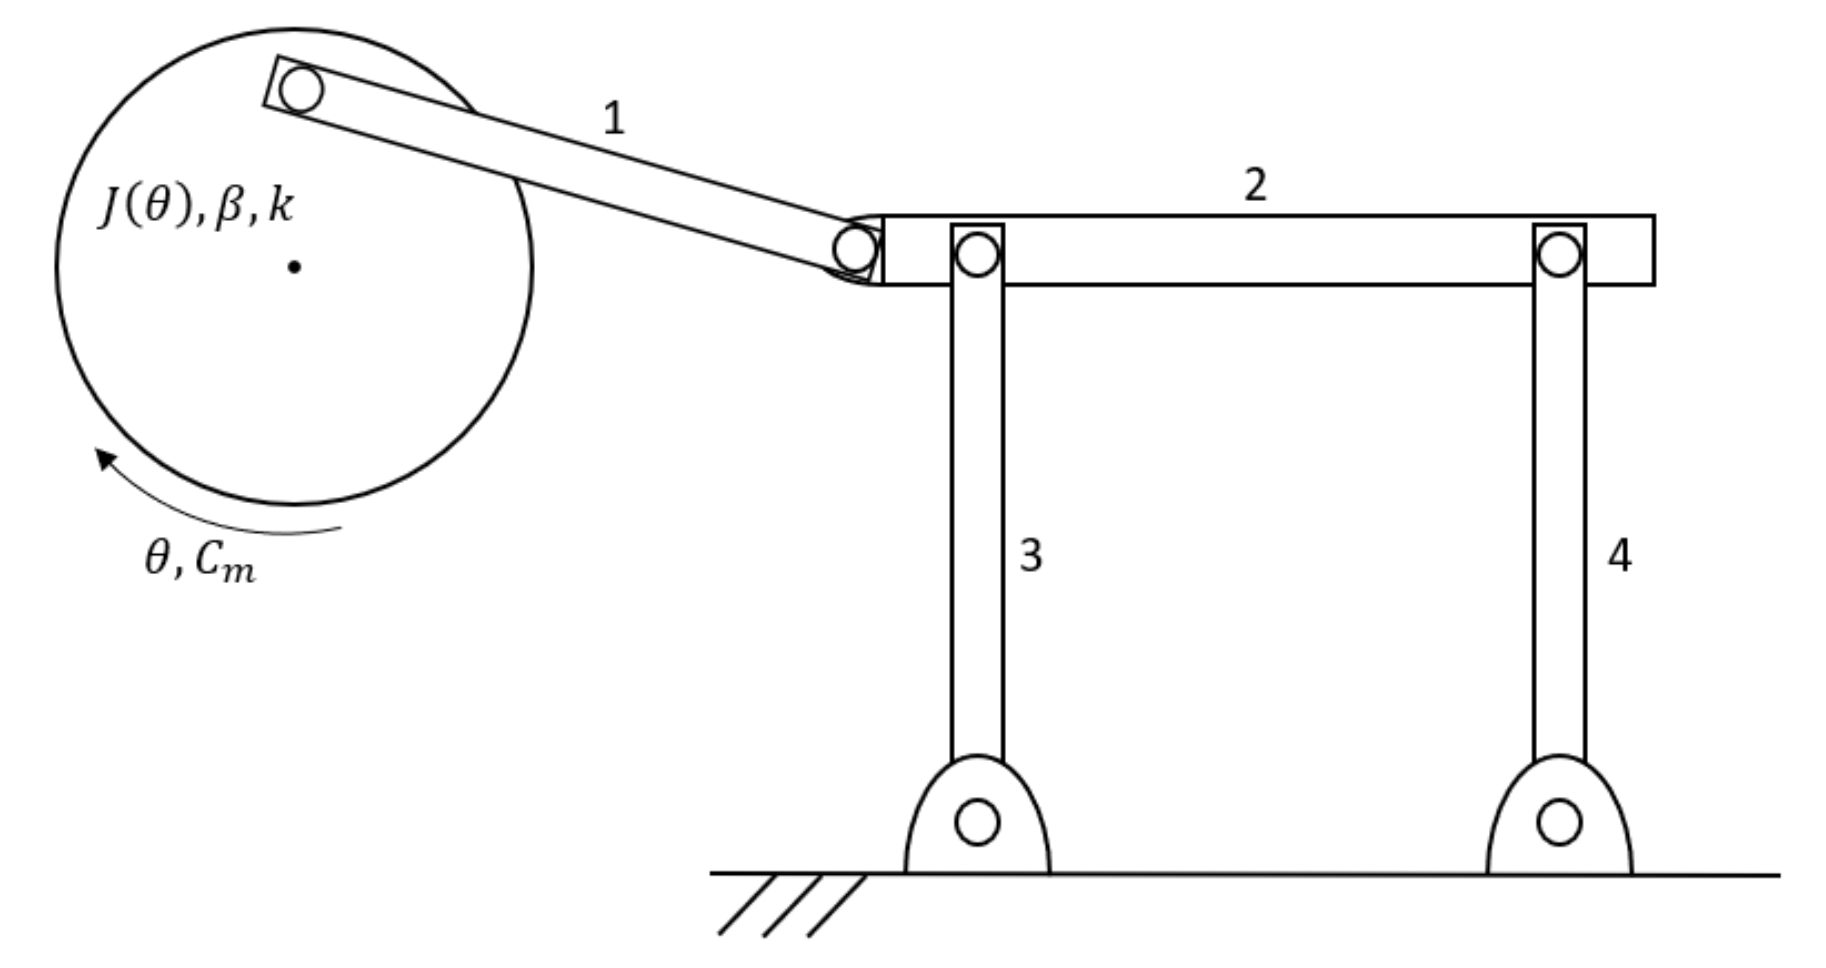
\includegraphics[width=0.75\linewidth]{./images/system_image.png}
	\caption{Schema illustrativo del sistema meccanismo motorizzato.}
	\label{fig:system_image}
\end{figure}
\section{Espressione del sistema in forma di stato e calcolo del sistema linearizzato intorno ad una coppia di equilibrio}

Innanzitutto, esprimiamo il sistema~\eqref{eq:system} nella seguente forma di stato
%
\begin{subequations}
	\begin{align}\label{eq:state_form}
		\dot{x} & = f(x,u)
		\\
		y       & = h(x,u).
	\end{align}
\end{subequations}
%
Pertanto, andiamo individuare lo stato $x$, l'ingresso $u$ e l'uscita $y$ del sistema come segue 
%
\begin{align*}
	x := \left [ \theta, \omega \right ]^T, \quad u := C_m , \quad y := \theta.
\end{align*}
%
Coerentemente con questa scelta, ricaviamo dal sistema~\eqref{eq:system} la seguente espressione per le funzioni $f$ ed $h$
%
\begin{align}
	f(x,u) & := 
	\begin{bmatrix}
		f_1(x,u)
		\\[0.5em] 
		f_2(x,u)
	\end{bmatrix} :=
	\begin{bmatrix}
		x_2
		\\[0.5em] 
		\dfrac{u - \beta x_2 - kx_1}{J(x_1)}
	\end{bmatrix}
	\\[0.5em] 
	h(x,u) & := x_1
\end{align}
%
Una volta calcolate $f$ ed $h$ esprimiamo~\eqref{eq:system} nella seguente forma di stato
%
\begin{subequations}\label{eq:our_system_state_form}
	\begin{align}
		\begin{bmatrix}
			\dot{x}_1
			\\
			\dot{x}_2
		\end{bmatrix} & = 
		\begin{bmatrix}
			f_1(x,u)
			\\[0.5em] 
			f_2(x,u)
		\end{bmatrix}\label{eq:state_form_1}
		\\[0.5em]
		y               & = h(x, u)
	\end{align}
\end{subequations}
%
Per trovare la coppia di equilibrio $(x_e, u_e)$ di~\eqref{eq:our_system_state_form}, andiamo a risolvere il seguente sistema di equazioni a partire dal valore fornito di $\theta_e=\frac{\pi}{3}$
%
\begin{align}
	\left\{\begin{matrix}
		       f(x_e, u_e)=0  
		       \\[0.5em]
		       x_{e1} = \frac{\pi}{3}
	       \end{matrix}\right.
\end{align}
%
dal quale otteniamo
%
\begin{align}
	x_e := \left[\frac{\pi}{3}, 0\right]^T,  \quad u_e = k\frac{\pi}{3}\label{eq:equilibirum_pair}
\end{align}
%
Definiamo le variabili alle variazioni $\delta x$, $\delta u$ e $\delta y$ come 
%
\begin{align*}
	\delta x & = x-x_e, 
	\quad
	\delta u = u-u_e, 
	\quad
	\delta y = y-y_e.
\end{align*}
%
L'evoluzione del sistema espressa nelle variabili alle variazioni pu\`o essere approssimativamente descritta mediante il seguente sistema lineare
%
\begin{subequations}\label{eq:linearized_system}
	\begin{align}
		\delta \dot{x} & = A_e\delta x + B_e\delta u
		\\
		\delta y       & = C_e\delta x + D_e\delta u,
	\end{align}
\end{subequations}
%
dove le matrici $A_e$, $B_e$, $C_e$ e $D_e$ vengono calcolate come
\\[0.5em]

\begin{subequations}\label{eq:matrices}\centering
	$A_e = \frac{\partial f(x, u)}{\partial x} \Bigg|_{\begin{smallmatrix}
			x = x_e
			\\
			u = u_e \end{smallmatrix}}$
	\quad
	$B_e = \frac{\partial f(x, u)}{\partial u} \Bigg|_{\begin{smallmatrix}
			x = x_e
			\\
			u = u_e \end{smallmatrix}}$
	\quad
	$C_e = \frac{\partial h(x, u)}{\partial x} \Bigg|_{\begin{smallmatrix}
			x = x_e
			\\
			u = u_e \end{smallmatrix}}$
	\quad
	$D_e = \frac{\partial h(x, u)}{\partial u} \Bigg|_{\begin{smallmatrix}
			x = x_e
			\\
			u = u_e \end{smallmatrix}}$
\end{subequations}
%
\section{Calcolo Funzione di Trasferimento}

In questa sezione, andiamo a calcolare la funzione di trasferimento $G(s)$ dall'ingresso $\delta u$ all'uscita $\delta y$ mediante la seguente formula 
%
%
\begin{align}\label{eq:transfer_function}
	G(s) = C(sI-A)^{-1}B + D = \frac{0.02}{1+0.09919\frac{s}{4.96}+\frac{s^2}{4.96^2}}
\end{align}
%
Dunque il sistema linearizzato~\eqref{eq:linearized_system} è caratterizzato dalla funzione di trasferimento~\eqref{eq:transfer_function} con 2 poli complessi coniugati $p_1$ e $p_2$:
\begin{align}
	p_1 = -0.2460 + 4.9536i, \quad p_2 = -0.2460 - 4.9536i
\end{align}
In Figura \ref{fig:G_bode} mostriamo il corrispondente diagramma di Bode. 

\begin{figure}[h!]
	\centering
	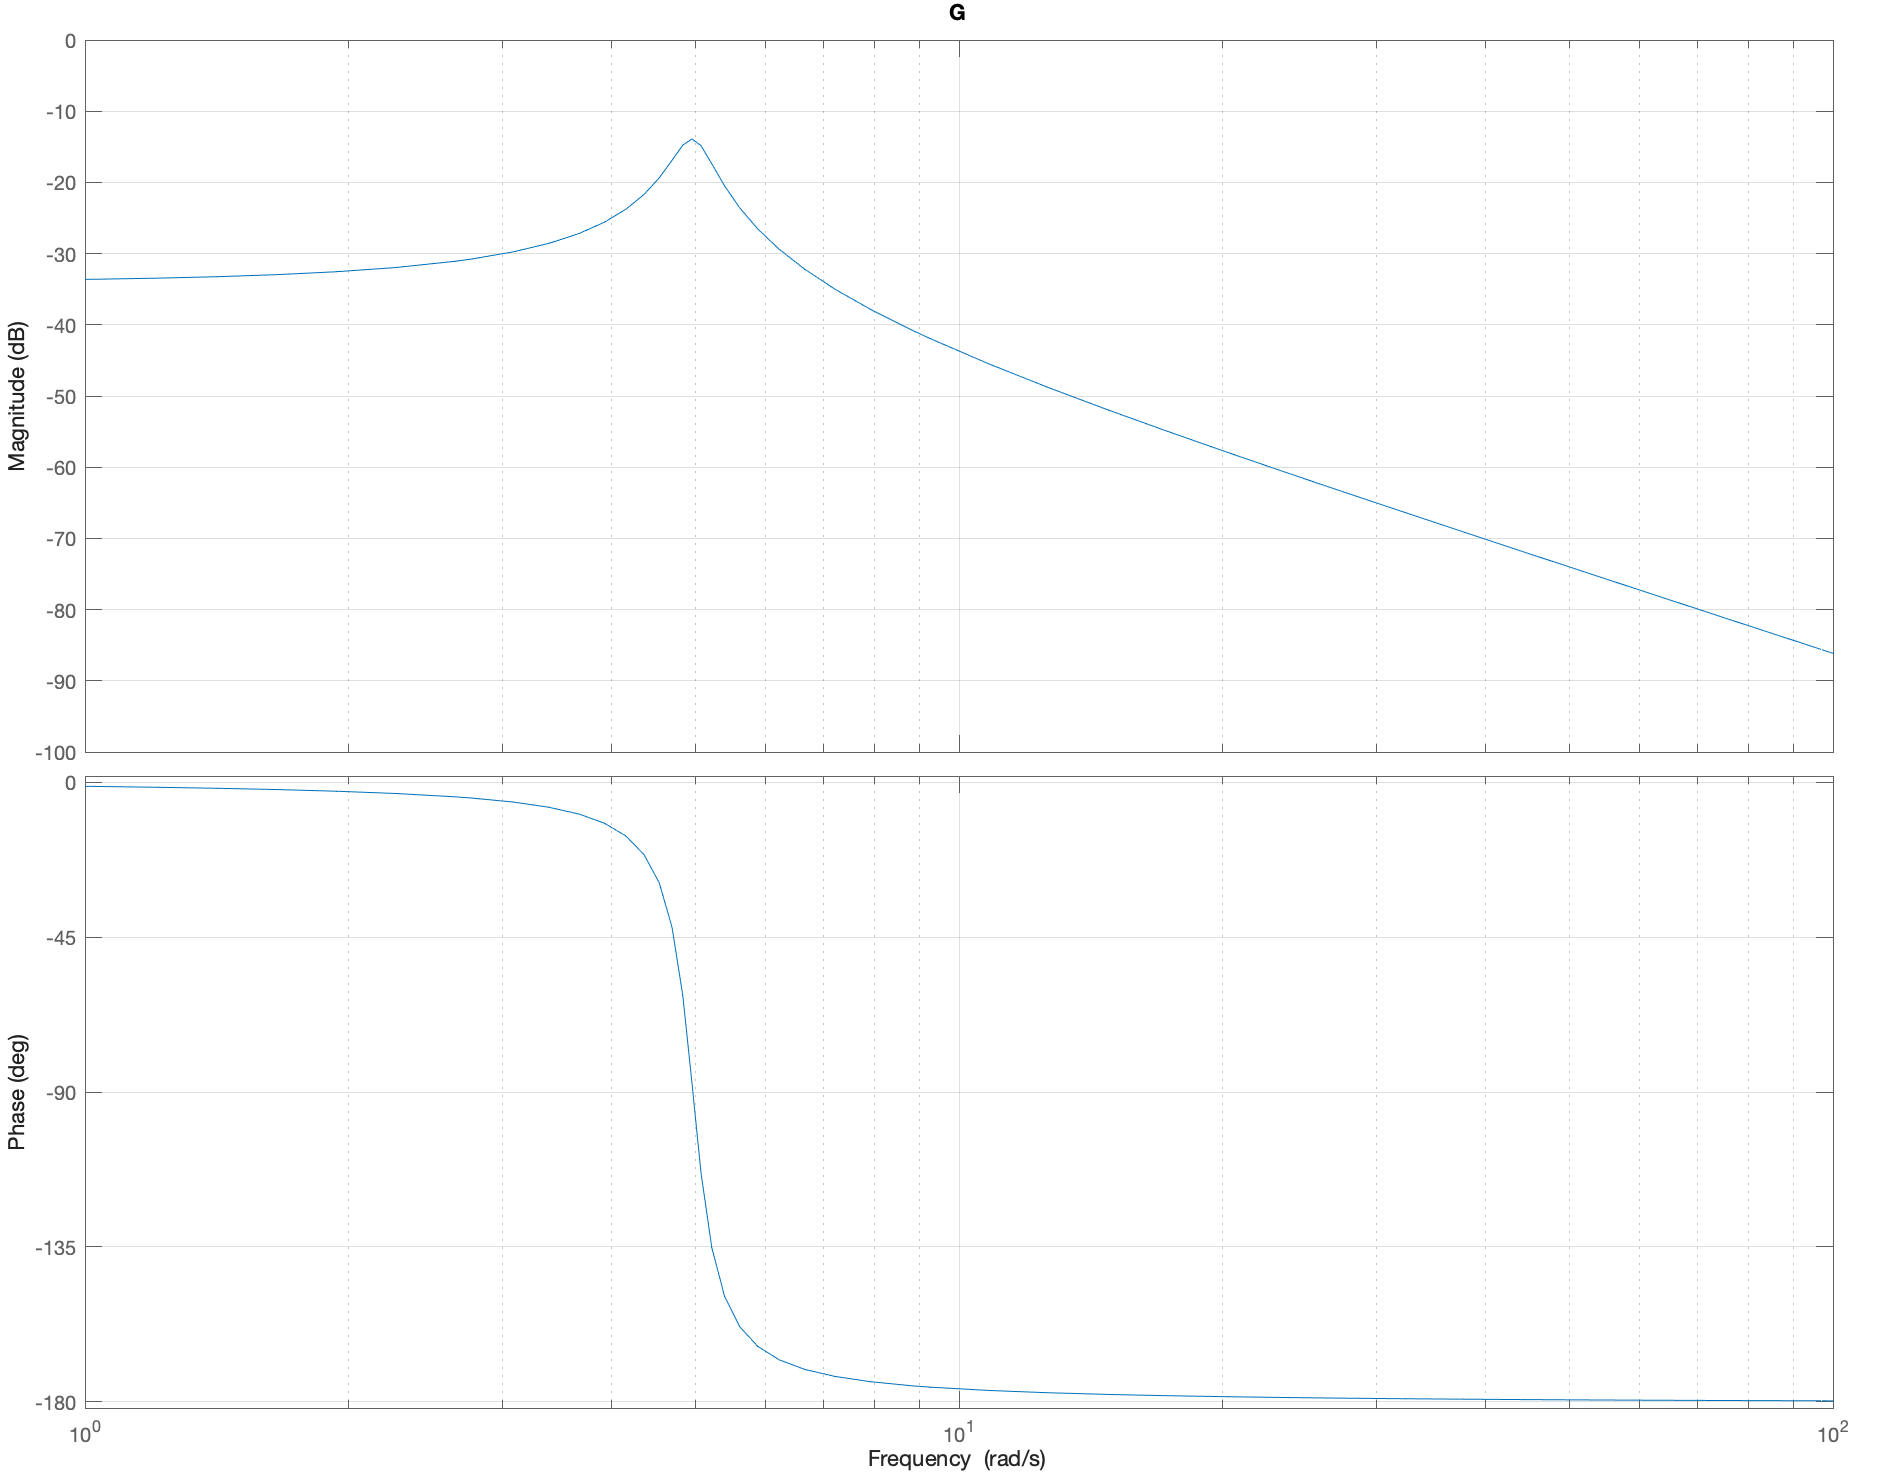
\includegraphics[width=0.75\linewidth]{./images/bode_G.png}
	\caption{Diagrammi di Bode della funzione di trasferimento G.}
	\label{fig:G_bode}
\end{figure}

\section{Mappatura specifiche del regolatore}
\label{sec:specifications}

Le specifiche da soddisfare sono
\begin{itemize}
	\item[1)] Errore a regime $|e_{\infty}| \leq e^{\star}$ in risposta a un gradino $\omega (t) = 1(t)$ e $d(t)=1(t)$
	\item[2)] Per garantire una certa robustezza del sistema si deve avere un margine di fase $M_f \geq 30^{\degree}$.
	\item[3)] Il sistema può accettare una sovraelongazione percentuale al massimo del 10\% : S\% $\leq 10\%$.
	\item[4)] Il tempo di assestamento alla $\epsilon_{\%}$ = 5\% deve essere inferiore al valore fissato: $T_{a, \epsilon} = 0.008s$ .
	\item[5)] Il disturbo sull'uscita d(t), con una banda limitata nel range di pulsazioni $[0, 0.5]$, deve essere abbattuto di almeno 30 dB.
	\item[6)] Il rumore sull'uscita n(t), con una banda limitata nel range di pulsazioni $[5 \cdot 10^4, 5 \cdot 10^6]$, deve essere abbattuto di almeno 65 dB.
\end{itemize}
%
Andiamo ad effettuare la mappatura punto per punto le specifiche richieste, tenendo a mente la fisica realizzabilità del regolatore.  

Pertanto, in Figura \ref{fig:G_bode_specifiche}, mostriamo il diagramma di Bode della funzione di trasferimento $G(s)$ con le zone proibite emerse dalla mappatura delle specifiche.
\begin{figure}[h!]
	\centering
	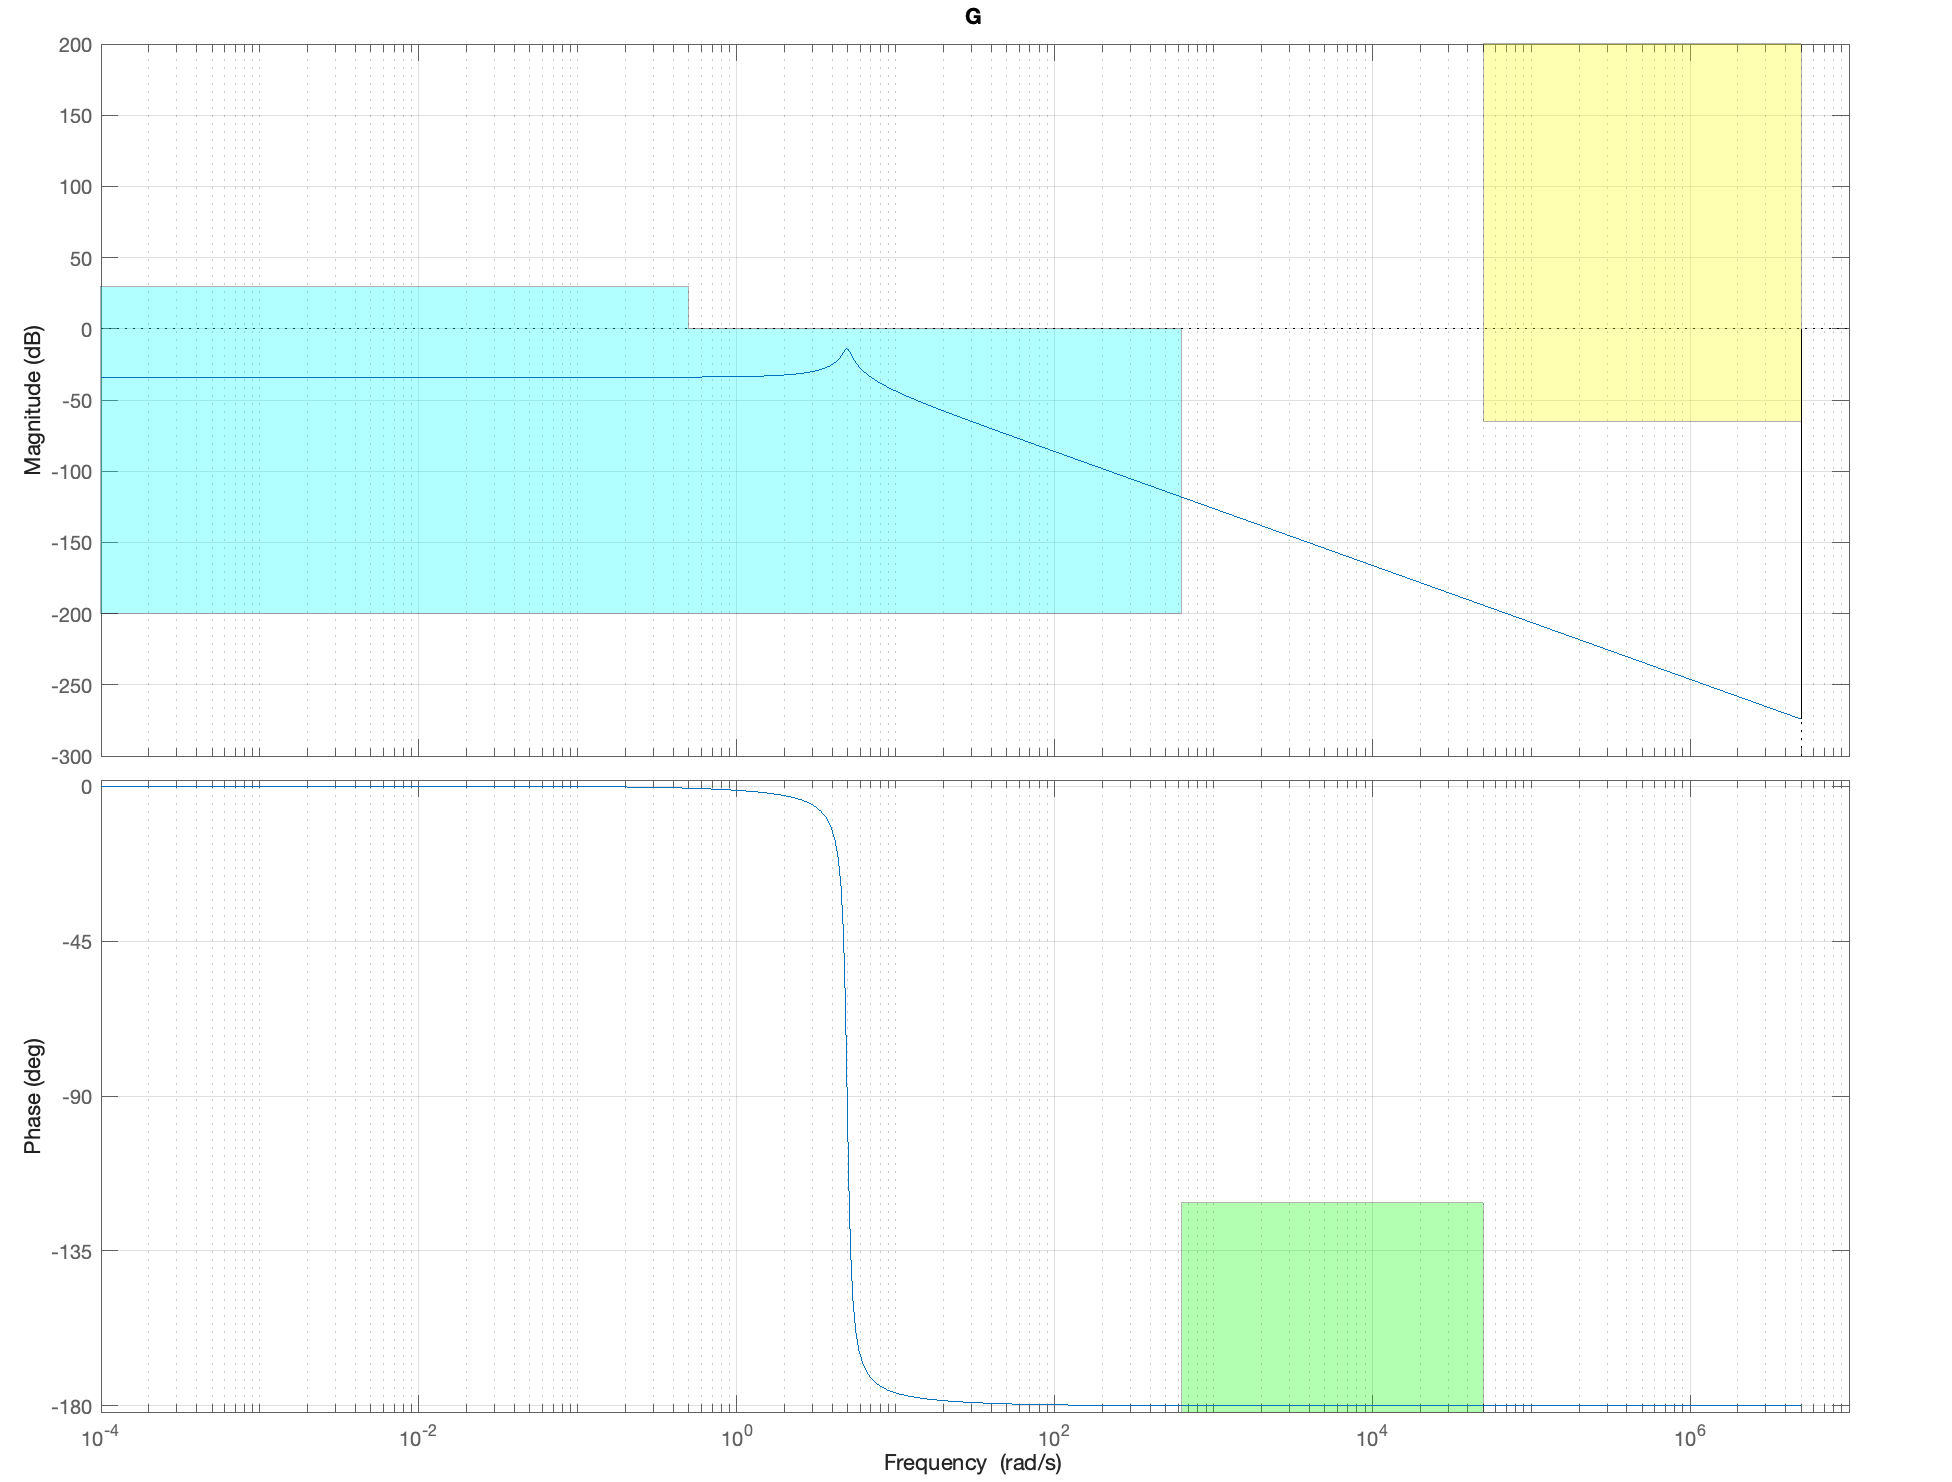
\includegraphics[width=0.75\linewidth]{./images/bode_G_mappatura.png}
	\caption{Mapputura delle specifiche.}
	\label{fig:G_bode_specifiche}
\end{figure}

\section{Sintesi del regolatore statico}
\label{sec:static_regulator}

In questa sezione progettiamo il regolatore statico $R_s(s)$ partendo dalle analisi fatte in sezione~\ref{sec:specifications}.

Nel nostro caso, essendo l'errore a regime $>$ 0 , possiamo progettare il regolatore statico come:
\begin{align}
	R(s) = \mu_s.
\end{align}

Consideriamo quindi che:
\begin{align}
	\mu_s \geq \mu^{\star} = \frac{D+W}{e^{\star}}.
\end{align}
Con D e W rispettive ampiezza dei gradini di disturbo sull'uscita e ingresso.\\
Per determinare $\mu_s$ bisogna anche considerare la specifica sull'attenuazione di d(t):
\begin{align}
	\mu_s \geq \mu_{sd} = 10^{\frac{A_d}{20}}.
\end{align}
Con $A_d$ pari a 30 dB. Otteniamo quindi $\mu_s$ come:
\begin{align}
	\mu_s \geq max\bigg(\frac{\mu^{\star}}{\left| L(0)\right|}, \frac{\mu_{sd}}{\left| G(j\omega_{d_{max}})\right|}\bigg).
\end{align}

Dunque, definiamo la funzione estesa $G_e(s) = R_s(s)G(s)$ e, in Figura \ref{fig:G_e}, mostriamo il suo diagramma di Bode per verificare se e quali zone proibite vengono attraversate.
Dalla figura emerge come il regolatore ora rispetti la specifica sull'attenuazione del disturbo in uscita.

\begin{figure}[h!]
	\centering
	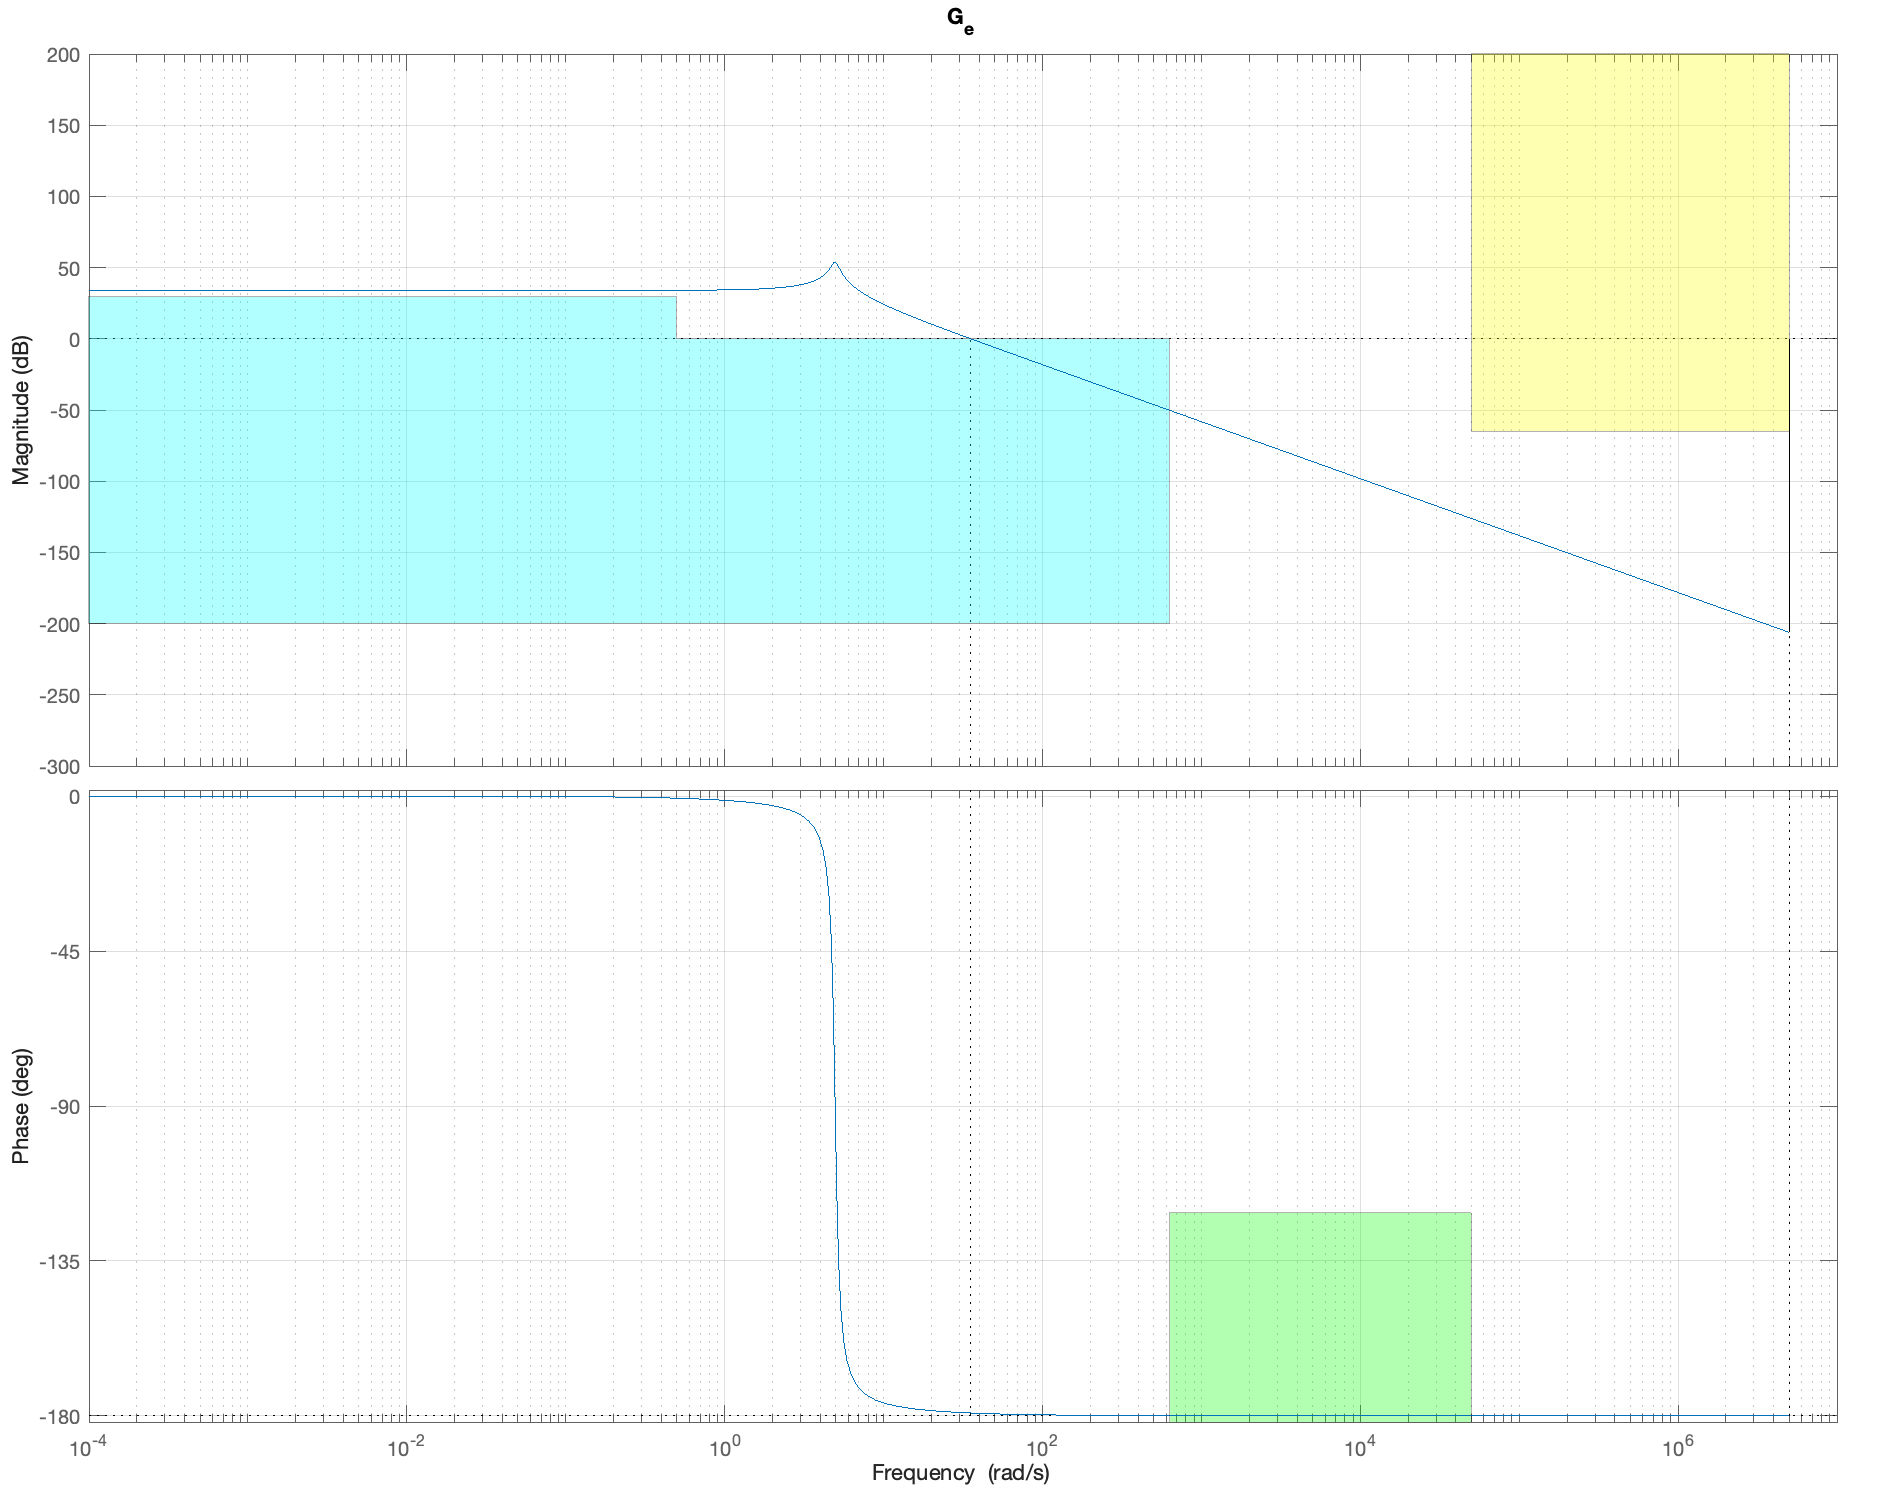
\includegraphics[width=0.75\linewidth]{./images/G_e.png}
	\caption{Mappatura specifiche su $G_e$.}
	\label{fig:G_e}
\end{figure}

\section{Sintesi del regolatore dinamico}
\label{sec:dynamic_regulator}

In questa sezione, progettiamo il regolatore dinamico $R_d(s)$. 
%
Dalle analisi fatte in Sezione~\ref{sec:static_regulator}, notiamo di essere nello Scenario di tipo B. Dunque, progettiamo $R_d(s)$ ricorrendo a una rete anticipatrice.\\
A questo scopo, calcoliamo il margine di fase per rispettare le specifiche:
\begin{align}
	\xi^{\star} = \sqrt{\frac{\log{S}^2}{\pi^2 + \log{S}^2}}.
	\\[0.5em]
	Mf = max (\xi^{\star}, 30).
\end{align}
Dove S=0.1. Otteniamo quindi:
\begin{align}
	\omega_{c_{min}}=\frac{300}{T_{a, 5}*Mf}.
\end{align}
La rete anticipatrice si presenta nella forma:
\begin{align}
	R_d(s) = \frac{1+\tau s}{1+\alpha \tau s}.
\end{align}
Nel nostro caso, sfruttando le formule di inversione:
\begin{align}
	\tau = \frac{M^{\star}-\cos{\varphi^{\star}}}{\omega_c^{\star}\sin{\varphi^{\star}}}, \quad
	\alpha = \frac{\cos{\varphi^{\star}-\frac{1}{M^{\star}}}}{\omega_c^{\star}\sin{\varphi^{\star}}}\frac{1}{\tau}.
	\\[1em]
	M^{\star} = 10^{-\frac{\left|G_e(j\omega_c^{\star})\right|_{dB}}{20}}, \quad
	\varphi^{\star} = M_f^{\star} -\pi - \angle{G_e(j\omega_c^{\star})},
\end{align}
con $\omega_c^{\star}$ pari a 750 $\frac{rad}{s}$ e $M_f^{\star}$ pari a $M_f + 5 \degree $, da noi fissati rispettando le specifiche.\\

In Figura \ref{fig:funzione_anello}, mostriamo il diagramma di Bode della funzione d'anello $L(s) = R_d(s) G_e(s)$

\begin{figure}[h!]
	\centering
	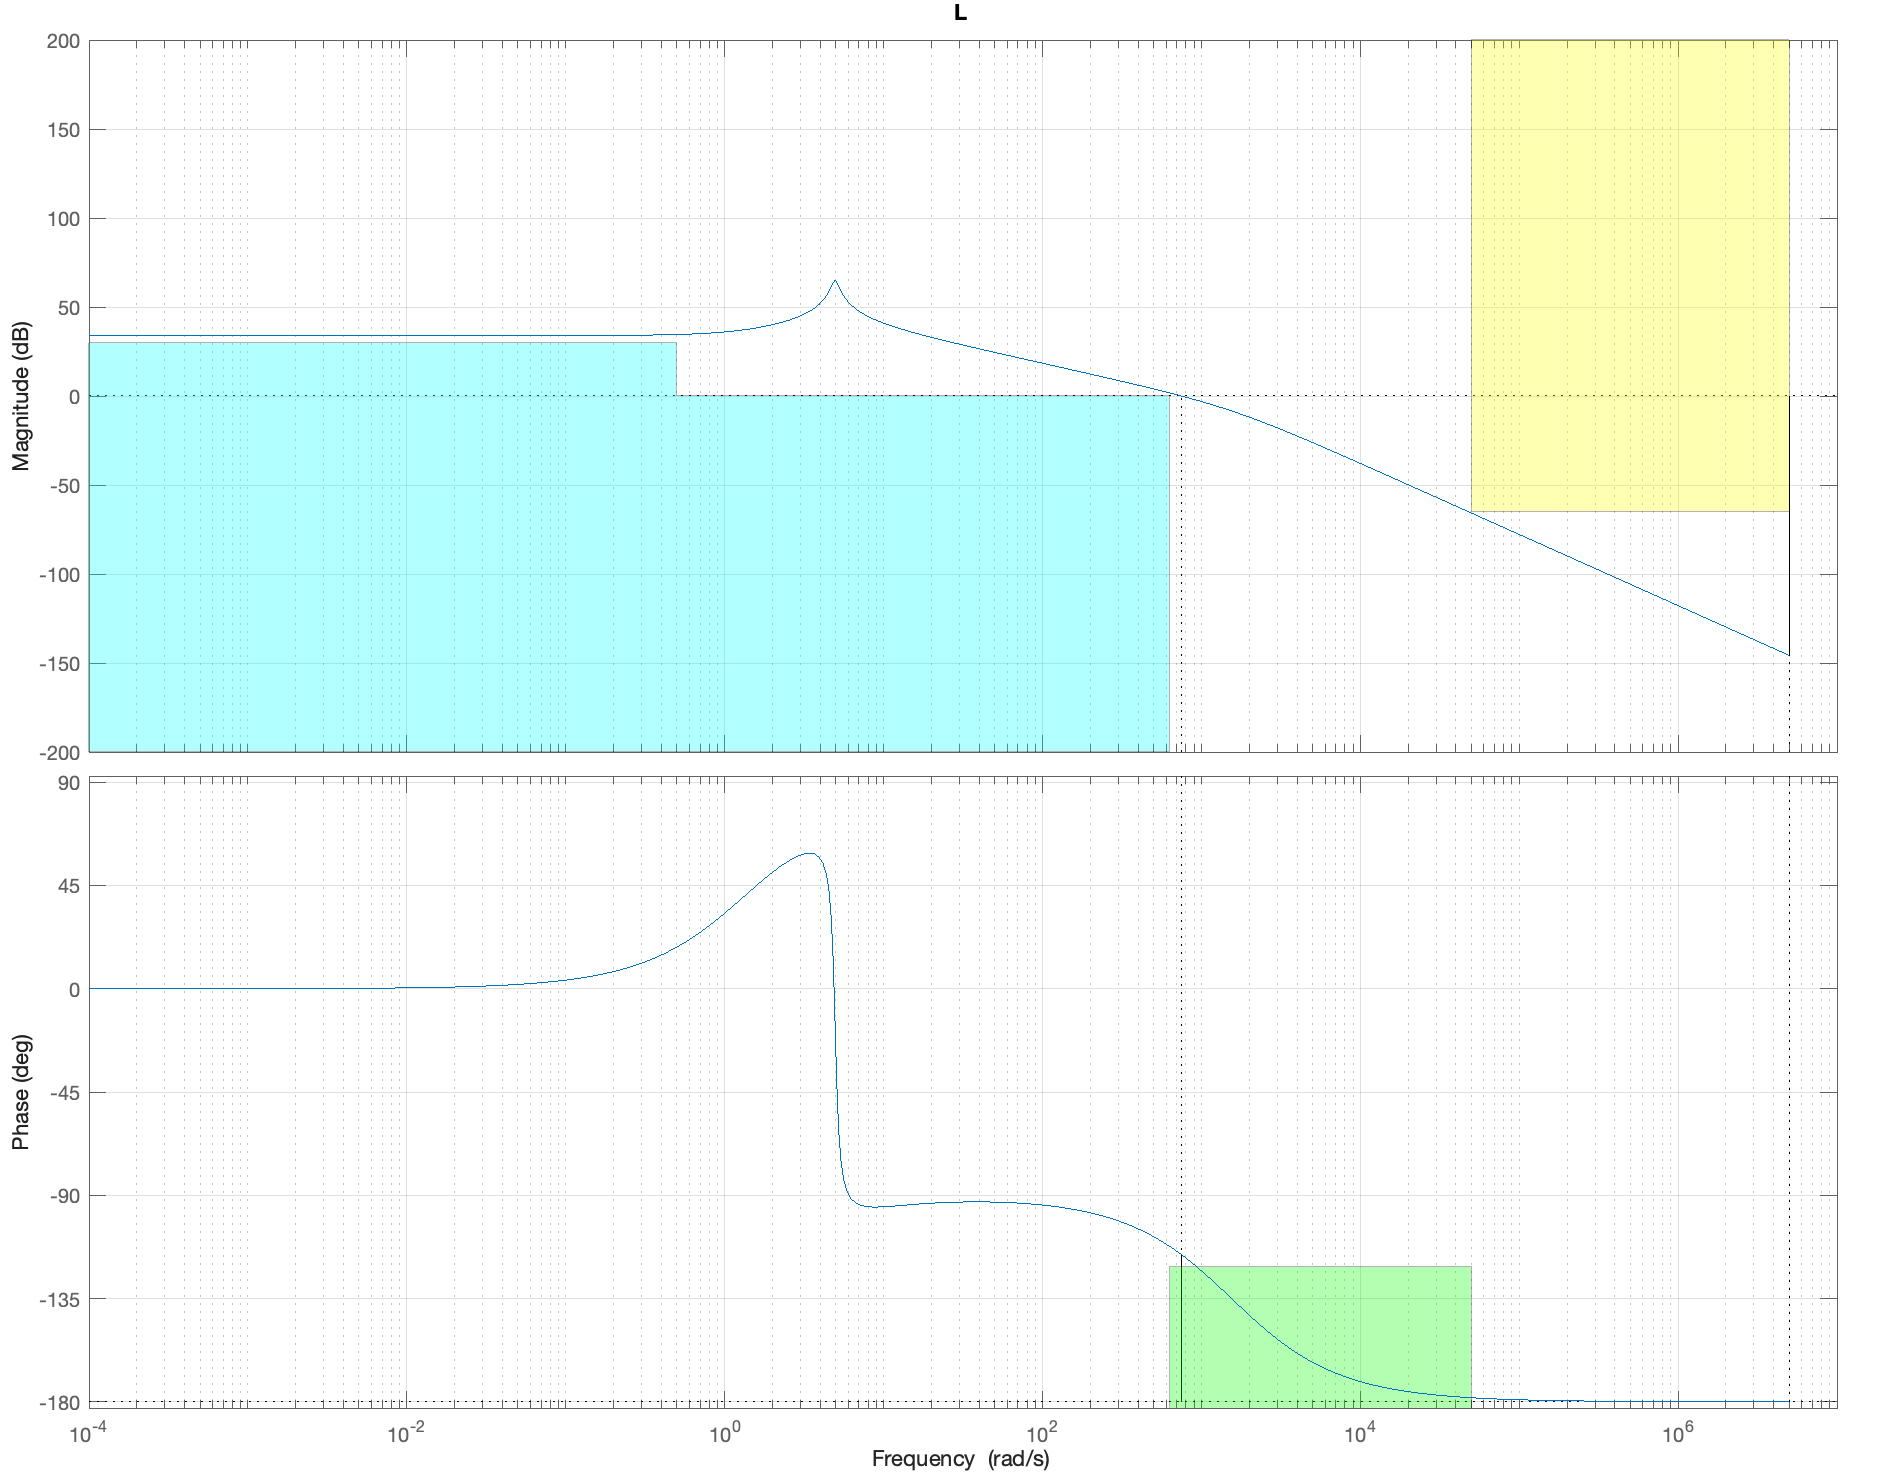
\includegraphics[width=0.75\linewidth]{./images/funzione_anello.png}
	\caption{Funzione d'anello L(s).}
	\label{fig:funzione_anello}
\end{figure}

\section{Test sul sistema linearizzato}

In questa sezione, testiamo l'efficacia del controllore progettato sul sistema linearizzato con $w(t) = 1(t)$, $d(t)=\sum_{k = 1}^{4} \sin(0.1kt)$ e $n(t)=\sum_{k = 1}^{4} \sin(5\space\cdot\space 10^{4}kt) $.

In Figura \ref{fig:step_response}, si mostra la risposta del sistema linearizzato ad un gradino unitario. \`E possibile notare come essa rispetti le specifiche richieste riguardanti tempo di assestamento, sovraelongazione e massimo errore a regime. 

Il grafico della risposta al gradino unitario non interseca né la patch rossa, che corrisponde a valori per cui non sarebbe rispettato il vincolo sulla sovraelongazione,
né la patch verde, la quale corrisponde a valori per cui il vincolo sul tempo di assestamento risulterebbe non rispettato. 
Inoltre, la risposta al gradino unitario a regime si stabilizza a $0.9804$, valore che ricade entro l'intervallo di errore di $\pm0.04$ richiesto dalle specifiche.

\begin{figure}[h!]
	\centering
	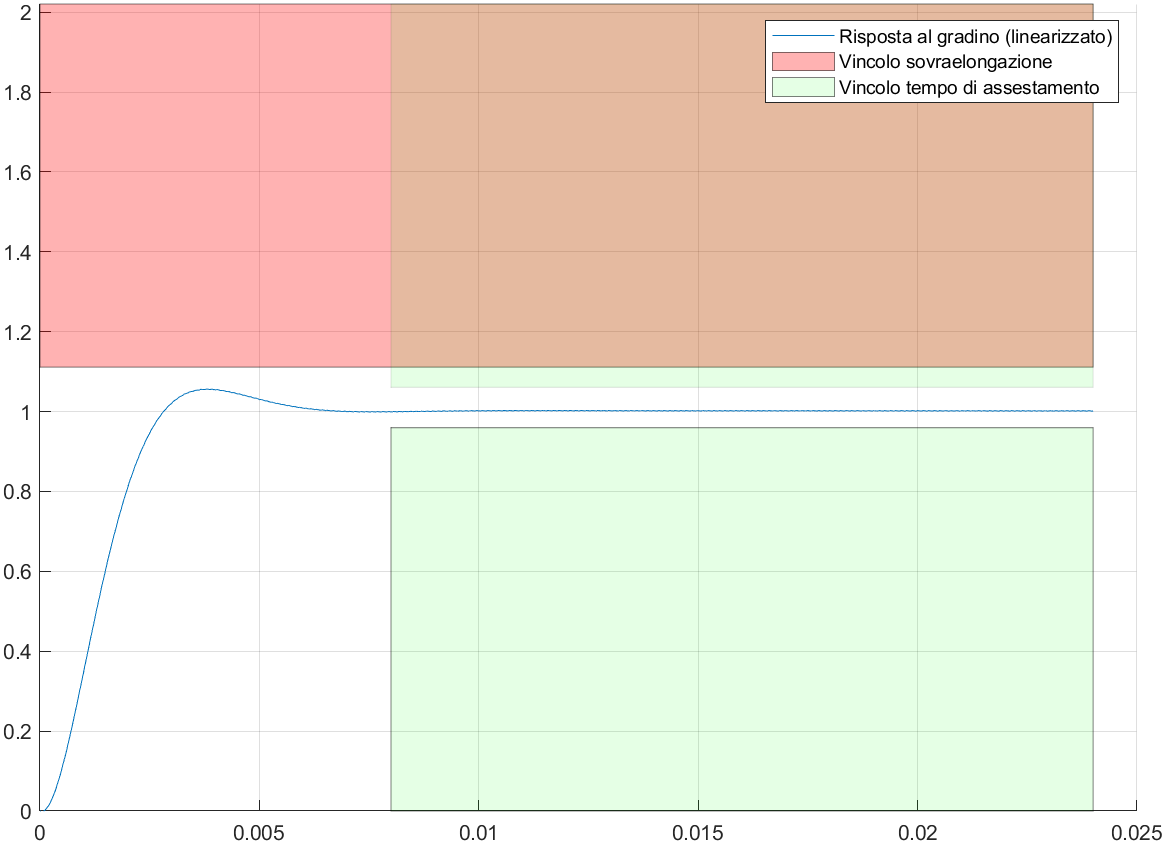
\includegraphics[width=0.75\linewidth]{./images/stepRespLin.png}
	\caption{Risposta del sistema linearizzato ad un gradino unitario.}
	\label{fig:step_response}
\end{figure}

Questo risultato \`e stato ottenuto progettando un regolatore statico $R_s(s)$ adeguato al fine di mantenere l'errore a regime inferiore ad un valore di $0.04$ (come spiegato nella Sezione~\ref{sec:static_regulator}) 
e un regolatore dinamico $R_d(s)$ che facesse s\`i che il sistema rispettasse un vincolo sul margine di fase $M_f$ tale per cui non si verificassero sovraelongazione e tempo di assestamento superiori alle specifiche richieste
(come spiegato nella Sezione~\ref{sec:dynamic_regulator}).

\section{Test sul sistema non lineare}

In questa sezione, testiamo l'efficacia del controllore progettato sul modello non lineare, tenendo anche conto della presenza di $d(t)$ ed $n(t)$. 
Il test \`e stato effettuato utilizzando un modello Simulink, come mostrato nella figura \ref*{fig:simulink}.

Pi\`u nello specifico,
da sinistra a destra si trovano un blocco generatore di segnali a gradino al quale viene sottratto il valore dell'uscita precedente (in modo da realizzare il controllo in retroazione), ed in seguito anche il disturbo di misura $n(t)$. 
Tutto ci\`o viene portato in ingresso ad un blocco Simulink contenente le specifiche del regolatore da noi definito, il cui output viene sommato al valore dell'ingresso all'equilibrio ($u_e$) e mandato in input ad un blocco contenente
le equazioni di stato del modello non lineare. L'uscita di quest'ultimo viene fatta passare per un blocco integratore in modo da ricavare in valore dello stato (il blocco precedente ha come valore di output $\dot{x}$). Il valore cos\`i ottenuto 
viene moltiplicato per il guadagno (matrice $C_e\cdot u$) e a quest'ultimo viene sommato il disturbo d'uscita $d(t)$, ottenendo cos\`i l'uscita del sistema non lineare, la quale viene portata in ingresso ad un blocco visualizzatore e fatta entrare nella retroazione,
dove le viene sottratto il valore di $x_e$, ossia l'equilibrio per lo stato. Quest'ultimo passaggio è realizzato per far sì che $x(t)$ converga a $x_e$.


\begin{figure}[h!]
	\centering
	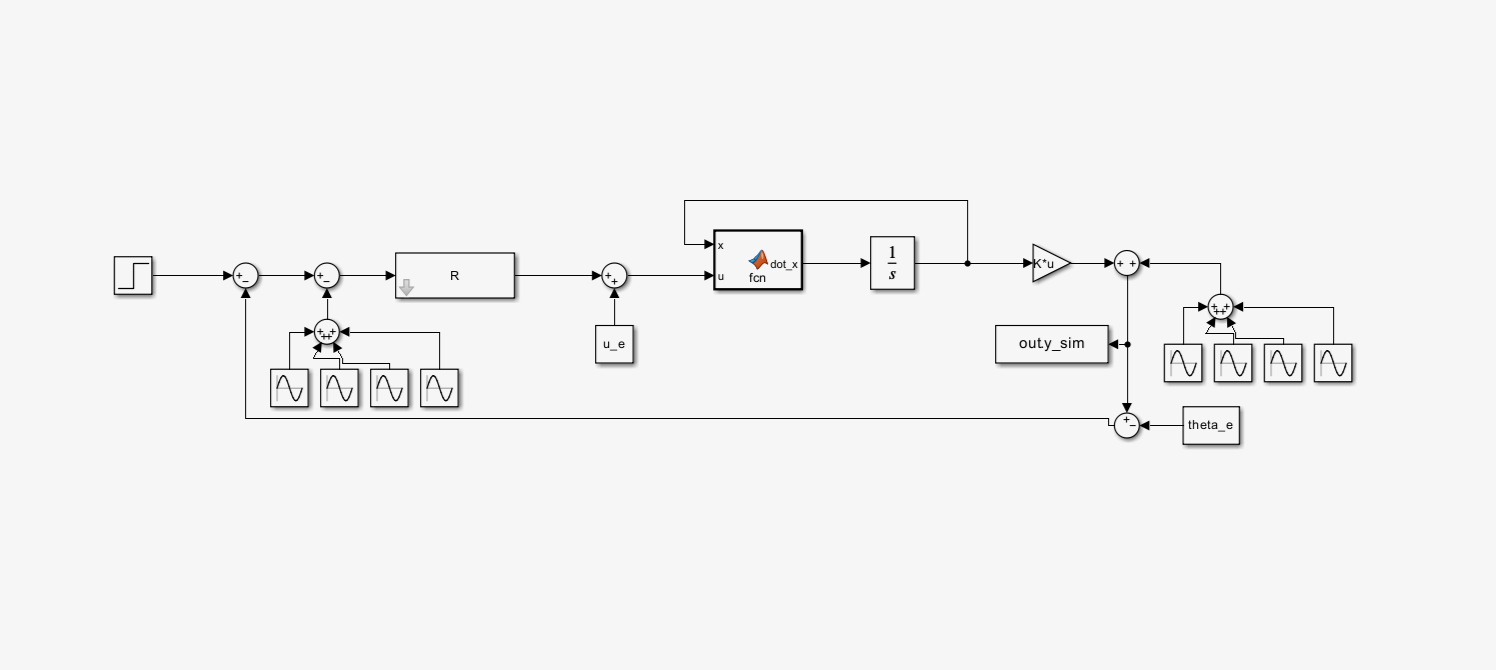
\includegraphics[width=0.75\linewidth]{./images/simulink1.png}
	\caption{Modello Simulink.}
	\label{fig:simulink}
\end{figure}

Nella figura \ref*{fig:step_response_non_lin_uni} si mostra la risposta del sistema non lineare ad un gradino unitario, calcolata utilizzando il sistema spiegato in precedenza (figura \ref*{fig:simulink}).

Si nota immediatamente come essa vada ad intersecare le patch sia rossa che verde. Ciò accade perché il regolatore è progettato sul sistema linearizzato, il quale non cattura il comportamento non lineare del sistema
e questo non ci assicura che il sistema non lineare rispetti precisamente le specifiche imposte per il sistema linearizzato.

\begin{figure}[h!]
	\centering
	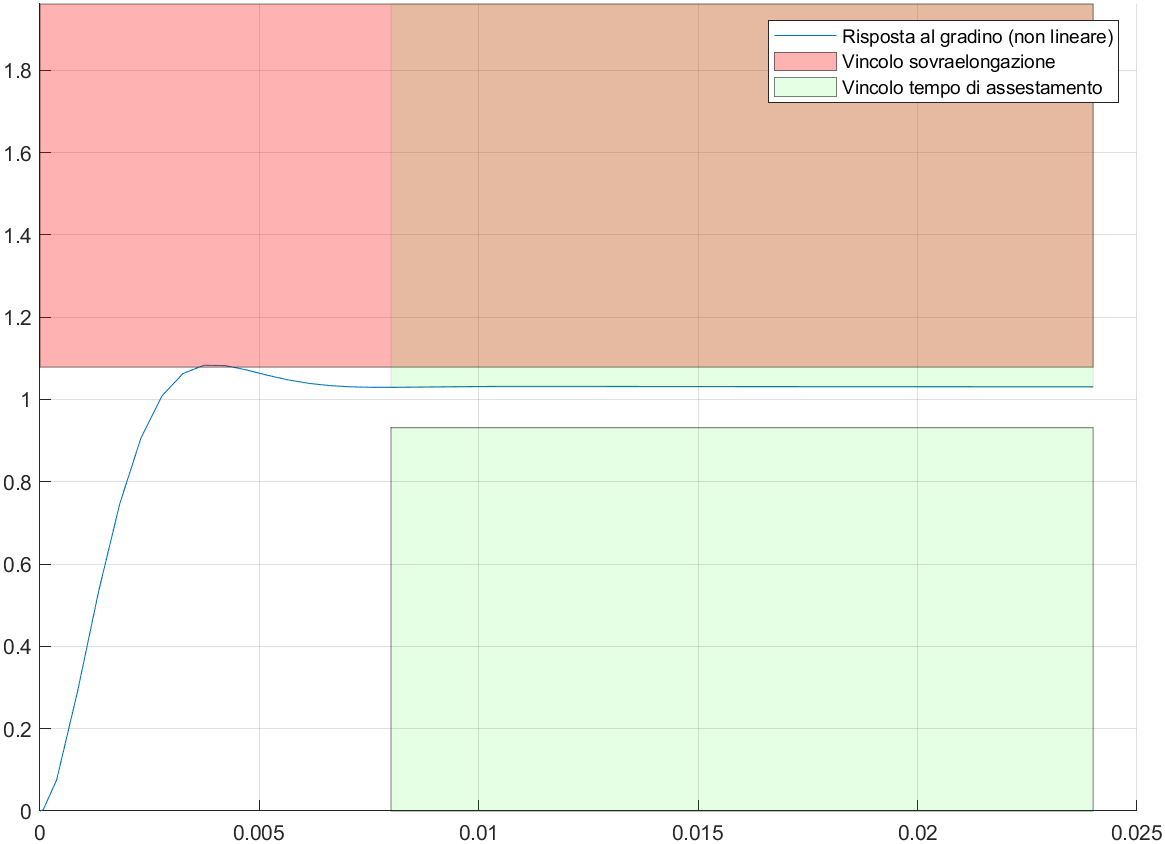
\includegraphics[width=0.75\linewidth]{./images/stepRespNonLinUni.png}
	\caption{Risposta del sistema non lineare ad un gradino unitario.}
	\label{fig:step_response_non_lin_uni}
\end{figure}

Nella figura \ref*{fig:confronto} è possibile osservare come, per tempi brevi, la risposta al gradino del sistema linearizzato e del sistema non lineare (sia in presenza che in assenza di disturbi) siano molto simili.
Ciò non si verifica nel caso di tempi più lunghi, dove la presenza di disturbi porta l'uscita del sistema non lineare a divergere dal riferimento, assumendo un comportamento non stabile - cosa che non avviene in assenza di distubi -
come mostrato nella figura \ref*{fig:confrontoReg}.

\begin{figure}[h!]
	\centering
	\begin{subfigure}[b]{0.45\textwidth}
		\centering
		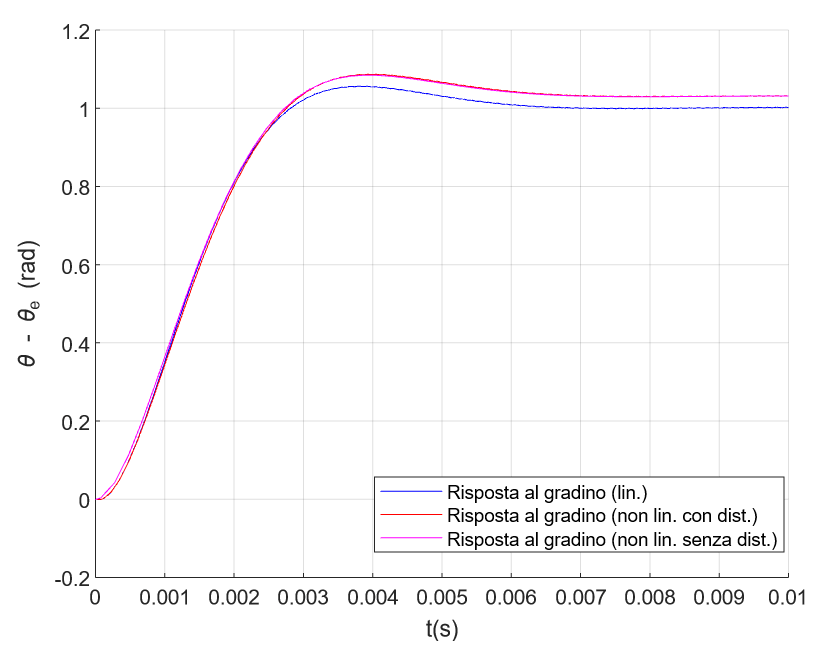
\includegraphics[width=\textwidth]{./images/confronto.png}
		\caption{Andamento della risposta al gradino per $0\leq t\leq 0.01$}
		\label{fig:confronto}
	\end{subfigure}
	\begin{subfigure}[b]{0.45\textwidth}
		\centering
		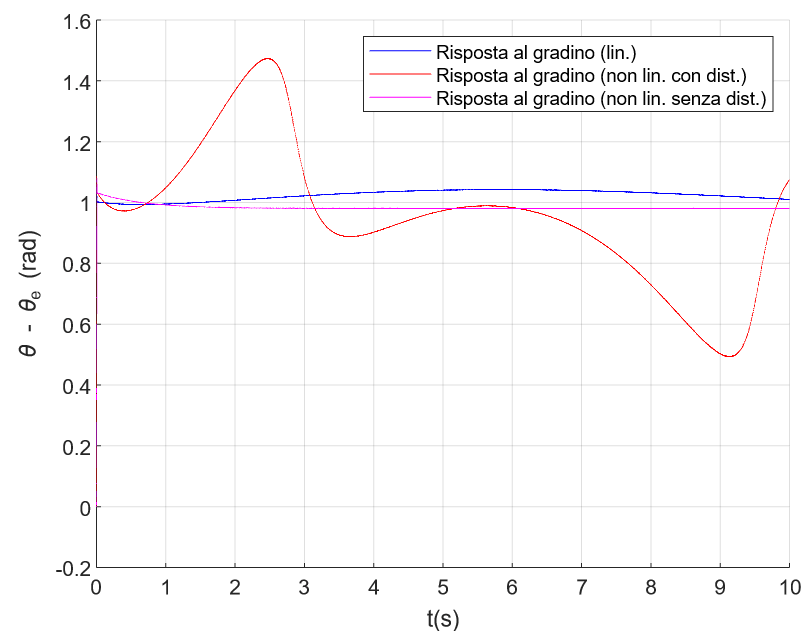
\includegraphics[width=\textwidth]{./images/confrontoReg.png}
		\caption{Andamento della risposta al gradino per $0\leq t\leq 10$}
		\label{fig:confrontoReg}
	\end{subfigure}
	
	\caption{}
	\label{fig:confronti}
\end{figure}

\section{Punti opzionali}

\subsection{Animazione}

L'animazione del sistema controllato è stata implementata in Matlab disegnando un grafico frame per frame in base all'angolo $\theta$ simulato.
Partendo da 3 posizioni fisse, ossia il centro della ruota(?) e i cardini(?) delle travi fissati al suolo, e in base all'angolo $\theta$ vengono calcolate le posizioni dei 3 cardini liberi.

In particolare si noti come i due cardini della trave(?) connessa alla ruota devono appartenere a due circonferenze. La prima è centrata chiaramente sul centro della ruota, per la seconda si noti che essendo il corpo rigido un parallelogramma, i tre cardini della trave orizzontale percorrono tutti delle circonferenze con raggio pari alla lunghezza delle travi verticali. È quindi possibile individuare una posizione univoca del secondo cardine in funzione della posizione del primo e della lunghezza della trave.

\begin{figure}[h!]
	\centering
	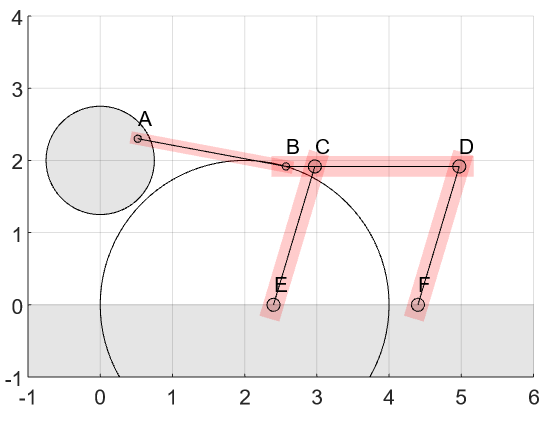
\includegraphics[width=0.4\linewidth]{./images/animazione_costruzione.png}
	\caption{Costruzione dei punti utilizzati per l'animazione}
	\label{fig:animazione_costruzione}
\end{figure}

\subsection{Secondo punto}

\begin{figure}[h!]
	\centering
	\begin{subfigure}[b]{0.4\textwidth}
		\centering
		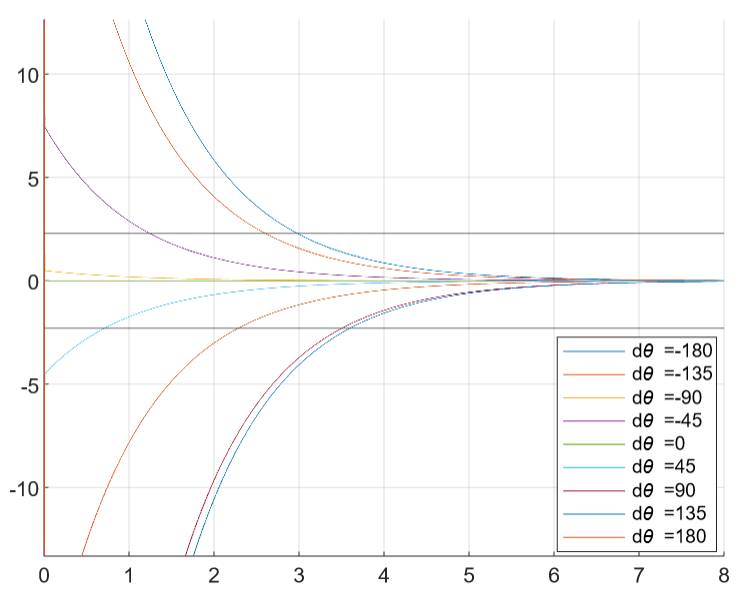
\includegraphics[width=\textwidth]{./images/theta_iniziali.png}
		\caption{Andamento di $\delta y$ al variare dell'angolo iniziale}
		\label{fig:theta_iniziali}
	\end{subfigure}
	\begin{subfigure}[b]{0.4\textwidth}
		\centering
		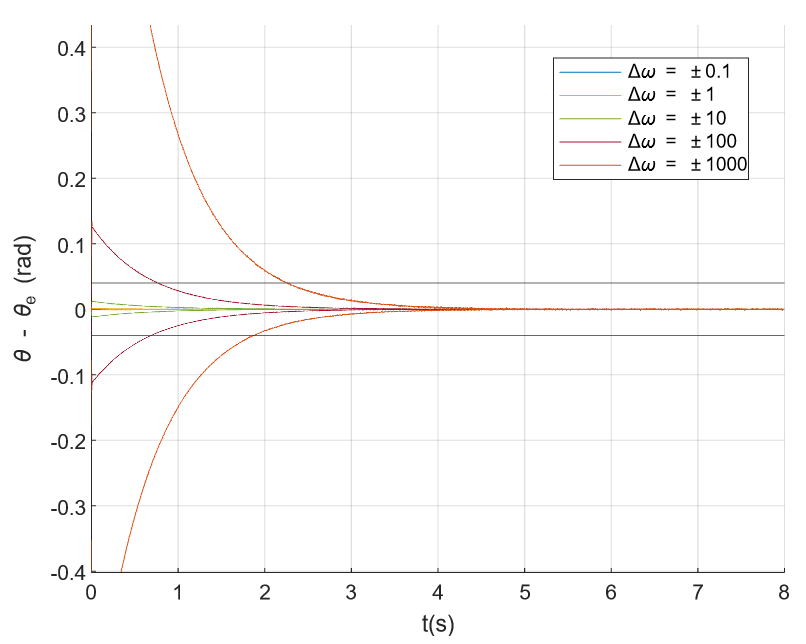
\includegraphics[width=\textwidth]{./images/omega_iniziali.png}
		\caption{Andamento di $\delta y$ al variare della velocità angolare iniziale, $0.1 \le \lvert\omega\rvert \le 10^6$}
		\label{fig:omega_iniziali}
	\end{subfigure}
	
	\caption{}
	\label{fig:stato_iniziale}
\end{figure}

Il regolatore realizzato è stato testato con un riferimento $\theta(t)=\theta_e$ sul sistema non lineare al variare dello stato iniziale. Essendo il regolatore progettato sul sistema linearizzato attorno a $\theta_e=\pi/3$, il riferimento in ingresso è data da $w(t)=\delta y=0$. Per variare lo stato iniziale del sistema è sufficiente variare lo stato iniziale dell'integratore in uscita al sistema dinamico nel modello in figura \ref{fig:simulink}.

Il sistema è considerato convergente al riferimento se soddisfa l'errore a regime di $e_{\infty} = 0.04$, analogamente alla progettazione del regolatore.

Il sistema non lineare rimane stabile e converge a $\theta_e$ per ogni variazione ragionevole dell'angolo e della velocità angolare iniziali, come mostrato nelle figure \ref{fig:theta_iniziali} e \ref{fig:omega_iniziali}.



\subsection{Terzo punto}

Per testare se il sistema non lineare controllato rispetta le specifiche in risposta a diversi gradini, sono necessarie due simulazioni. La prima, di lunga durata, controlla se la risposta rispetta l'errore a regime di 0.04. La seconda per verificare le prestazioni dinamiche delle risposte.
Per quanto riguarda la precisione dinamica i gradini nell'intervallo [1.1, 1.4) rispettano i vincoli di sovraelungazione e tempo di assestamento al 5\%(figure \ref{fig:gradini_dinamico_low} e \ref{fig:gradini_dinamico_high}).
In questo intervallo tutti i gradini rispettano l'errore a regime, mostrato in figura \ref{fig:gradini_statico}.

\begin{figure}[h!]
	\centering
	\begin{subfigure}[b]{0.3\textwidth}
		\centering
		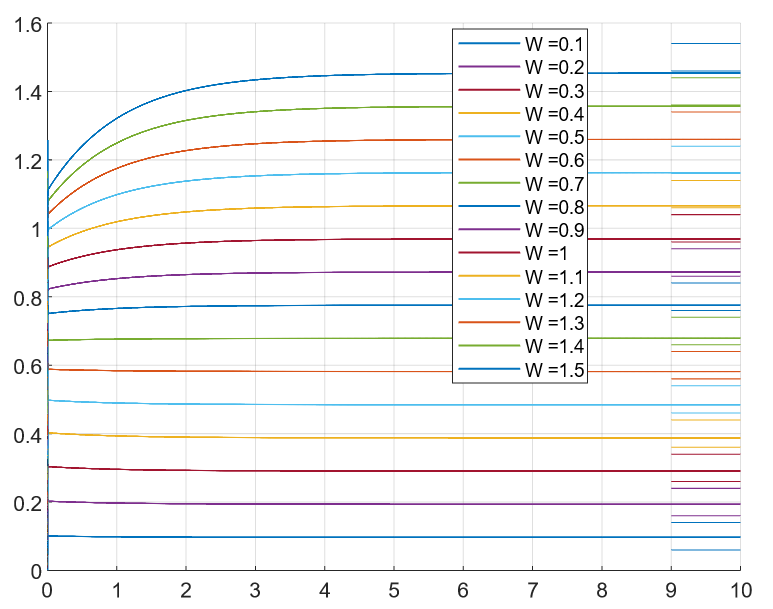
\includegraphics[width=\textwidth]{./images/gradini_statico.png}
		\caption{Precisione statica}
		\label{fig:gradini_statico}
	\end{subfigure}
	\begin{subfigure}[b]{0.3\textwidth}
		\centering
		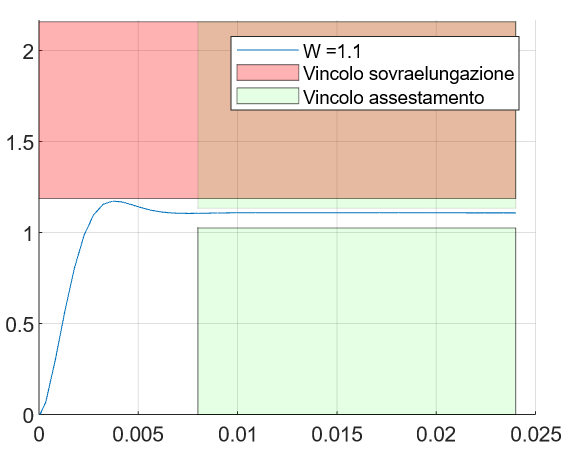
\includegraphics[width=\textwidth]{./images/gradini_dinamico_low.png}
		\caption{Precisione dinamica}
		\label{fig:gradini_dinamico_low}
	\end{subfigure}
	\begin{subfigure}[b]{0.3\textwidth}
		\centering
		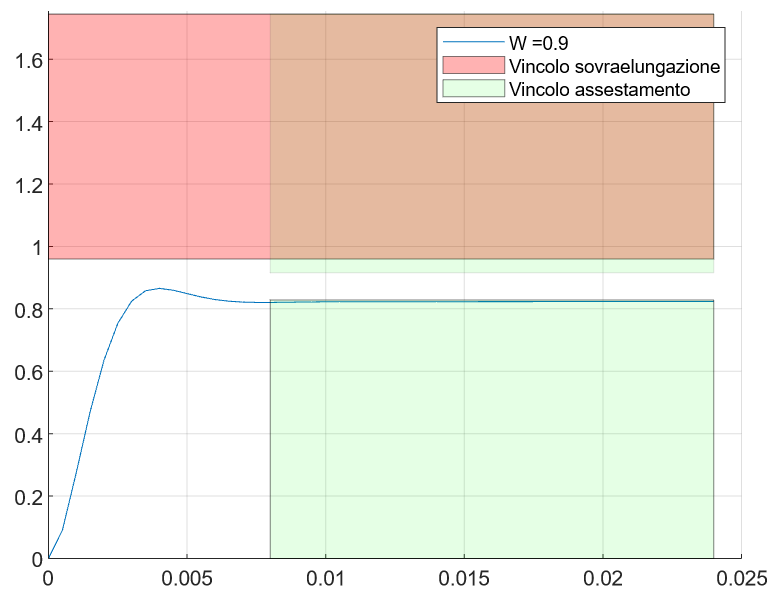
\includegraphics[width=\textwidth]{./images/gradini_dinamico_high.png}
		\caption{Precisione dinamica}
		\label{fig:gradini_dinamico_high}
	\end{subfigure}
	
	\caption{Verifica specifiche}
	\label{fig:specifiche_gradini}
\end{figure}

\section{Conclusioni}

In conclusione, sebbene il regolatore progettato sia efficiace e rispetti le specifiche sul sistema linearizzato, esso non offre le stesse prestazioni nel controllo del sistema non lineare. Non viene infatti rispettata le specifiche dinamiche sul tempo di assestamento al 5\% e sulla sovraelungazione per $w(t) = 1(t)$. Cioè è dovuto al comportamento non lineare del sistema, non catturabile nella linearizzazione, che porta a una differenza nell'inseguimento del riferimento.
Inoltre il regolatore non è in grado di attenuare correttamente i disturbi di misura nel sistema non lineare, il che porta l'uscita a divergere dal riferimento.
Il regolatore è però, in assenza di disturbi, in grado di riportare il sistema non lineare alle condizioni di equilibrio per ogni angolo e velocità inziale ragionevoli.
Inoltre, sebbene il controllo non sia efficace per un gradino di ampiezza $W=1$, lo diventa per tutti i gradini con ampiezza nel range $[1.1, 1.4)$.

\end{document}
